\documentclass[12pt]{article}
\usepackage[margin=2cm]{geometry}
\usepackage{titling}
\usepackage{graphicx}
\usepackage{float}
\usepackage[hidelinks]{hyperref}
\usepackage[italian]{babel}
\usepackage{subcaption}

\setlength\parindent{0pt}
\setlength{\parskip}{1em}
\setlength{\droptitle}{-2cm}

\title{Istruzioni d'uso ChocoPrinter}
\author{Università della Svizzera Italiana}
\date{Versione \today}


\begin{document}
\maketitle
\tableofcontents
\newpage

\section{Setup}

	\subsection{Download}\label{sec:download}

		Sono necessari i seguenti software:

		- Repetier-Host, \url{https://www.repetier.com/download-now}

		- Configurazioni per slicer, \url{https://github.com/USI-Showroom/ChocoPrinter/blob/master/config/Slic3r_config_choco.ini}

		Per aggiornare il firmware della stampante (opzionale):

		- Arduino IDE 1.0.6, \url{https://www.arduino.cc/en/Main/OldSoftwareReleases}

		- Firmware stampante (vedi sotto), \url{https://3dprint.elettronicain.it/blog/2012/09/06/software/}
		
		
	\subsection{Configurazione}\label{config}
	
		Installare il software Repetier-Host sulla propria macchina ed avviarlo. Cliccare sulla scheda \texttt{Slicer} e in seguito sul pulsante \texttt{Configure}. Cliccare su \texttt{Cancel} per chiudere la procedura guidata e dal menu \texttt{File} scegliere \texttt{Load Config}. Scegliere il file di configurazione (\texttt{Slic3r\_config\_choco.ini}) scaricato in precedenza.\\
		Cliccare sull'ingranaggio accanto al campo \texttt{Print settings}, poi sull'icona di salvataggio accanto al nome del profilo, salvarlo con il nome desiderato (p.es. "ChocoPrinter") e verificare i seguenti parametri:
		
		- Layers and perimeters $>$ Layer Height: 0.7mm\\
		- Infill $>$ FIll Density: 100\%\\
		- Speed $>$ Speed for print moves: 20 mm/s\\
		
		Se non ci sono errori, confermare con \texttt{Ok}. Chiudere la scheda e ripetere l'operazione con il campo \texttt{Filament}:

		- Filament $>$ Temperature ($^{\circ}$C) $>$ Extruder: 33\\
		- Filament $>$ Temperature ($^{\circ}$C) $>$ Bed: 0\\
		- Cooling $>$ Keep fan always on: On\\
		- Cooling $>$ Fan speed: 100
		
		Stessa cosa per il campo \texttt{Printer}. Al termine, chiudere la finestra \texttt{Slic3r} e scegliere i nuovi profili appena creati dal pannello \texttt{Slic3r} di Repetier-Host.\\
		
		Dalle icone in alto a destra cliccare su \texttt{Printer settings}; assicurarsi di aver scelto la porta corretta e di aver impostato la \texttt{Baud Rate} a 250000.


\section{Stampa}

	\begin{enumerate}
		\item Far partire il software Repetier-Host
	
		\item Cliccare su \texttt{Object Placement} e scegliere l'oggetto (file *.stl) da stampare tramite il pulsante \texttt{Add STL file}
	
		\item Modificare la dimensione dell'oggetto se necessario, modificando il valore del campo \texttt{Scale}

		\item Cliccare su \texttt{Slice with Slic3r}

		\item Accendere la stampante

		\item Collegarsi alla stampante tramite il cavo USB. Assicurarsi di avere configurato il software come descritto al punto \ref{config}

		\item Inserire il cioccolato fuso (preferibilmente di tipo ``Crémant") nella siringa
		
		\item Se necessario alzare il supporto girando la ruota bianca, per poter inserire correttamente la siringa. Qualora il motore dovesse fare resistenza, cliccare su \texttt{Stop Motor} dal pannello \texttt{Print Panel}

		\item Montare l'ago (2) e il tondino di alluminio (1) sulla siringa (3) e poi infilarla nel cilindro della stampante (4). Assicurarsi che il piatto di vetro (5) sia presente, pulito e ben tenuto dai quattro clip (6) sui lati (vedi immagine sottostante)

		\item Una volta che il cioccolato esca dalla siringa, cliccare su \texttt{Run} per avviare la stampa
	\end{enumerate}

	Durante la stampa verificare periodicamente che il cioccolato stia uscendo dalla siringa. È possibile mettere in pausa la stampante con il tasto \texttt{Pause} se necessario; dal pannello \texttt{Print Panel} è possibile avanzare o ritrarre lo stantuffo tramite i comandi \texttt{Extrude} e \texttt{Retract}. Non tentare di muovere o far forza su nessuna parte mobile quando la stampante è in pausa!\\
	
	\textbf{IMPORTANTE: NON} lasciare \textbf{mai} la stampante senza sorveglianza!\\
	
	\begin{figure}[H]
        \begin{subfigure}{0.5\textwidth}
                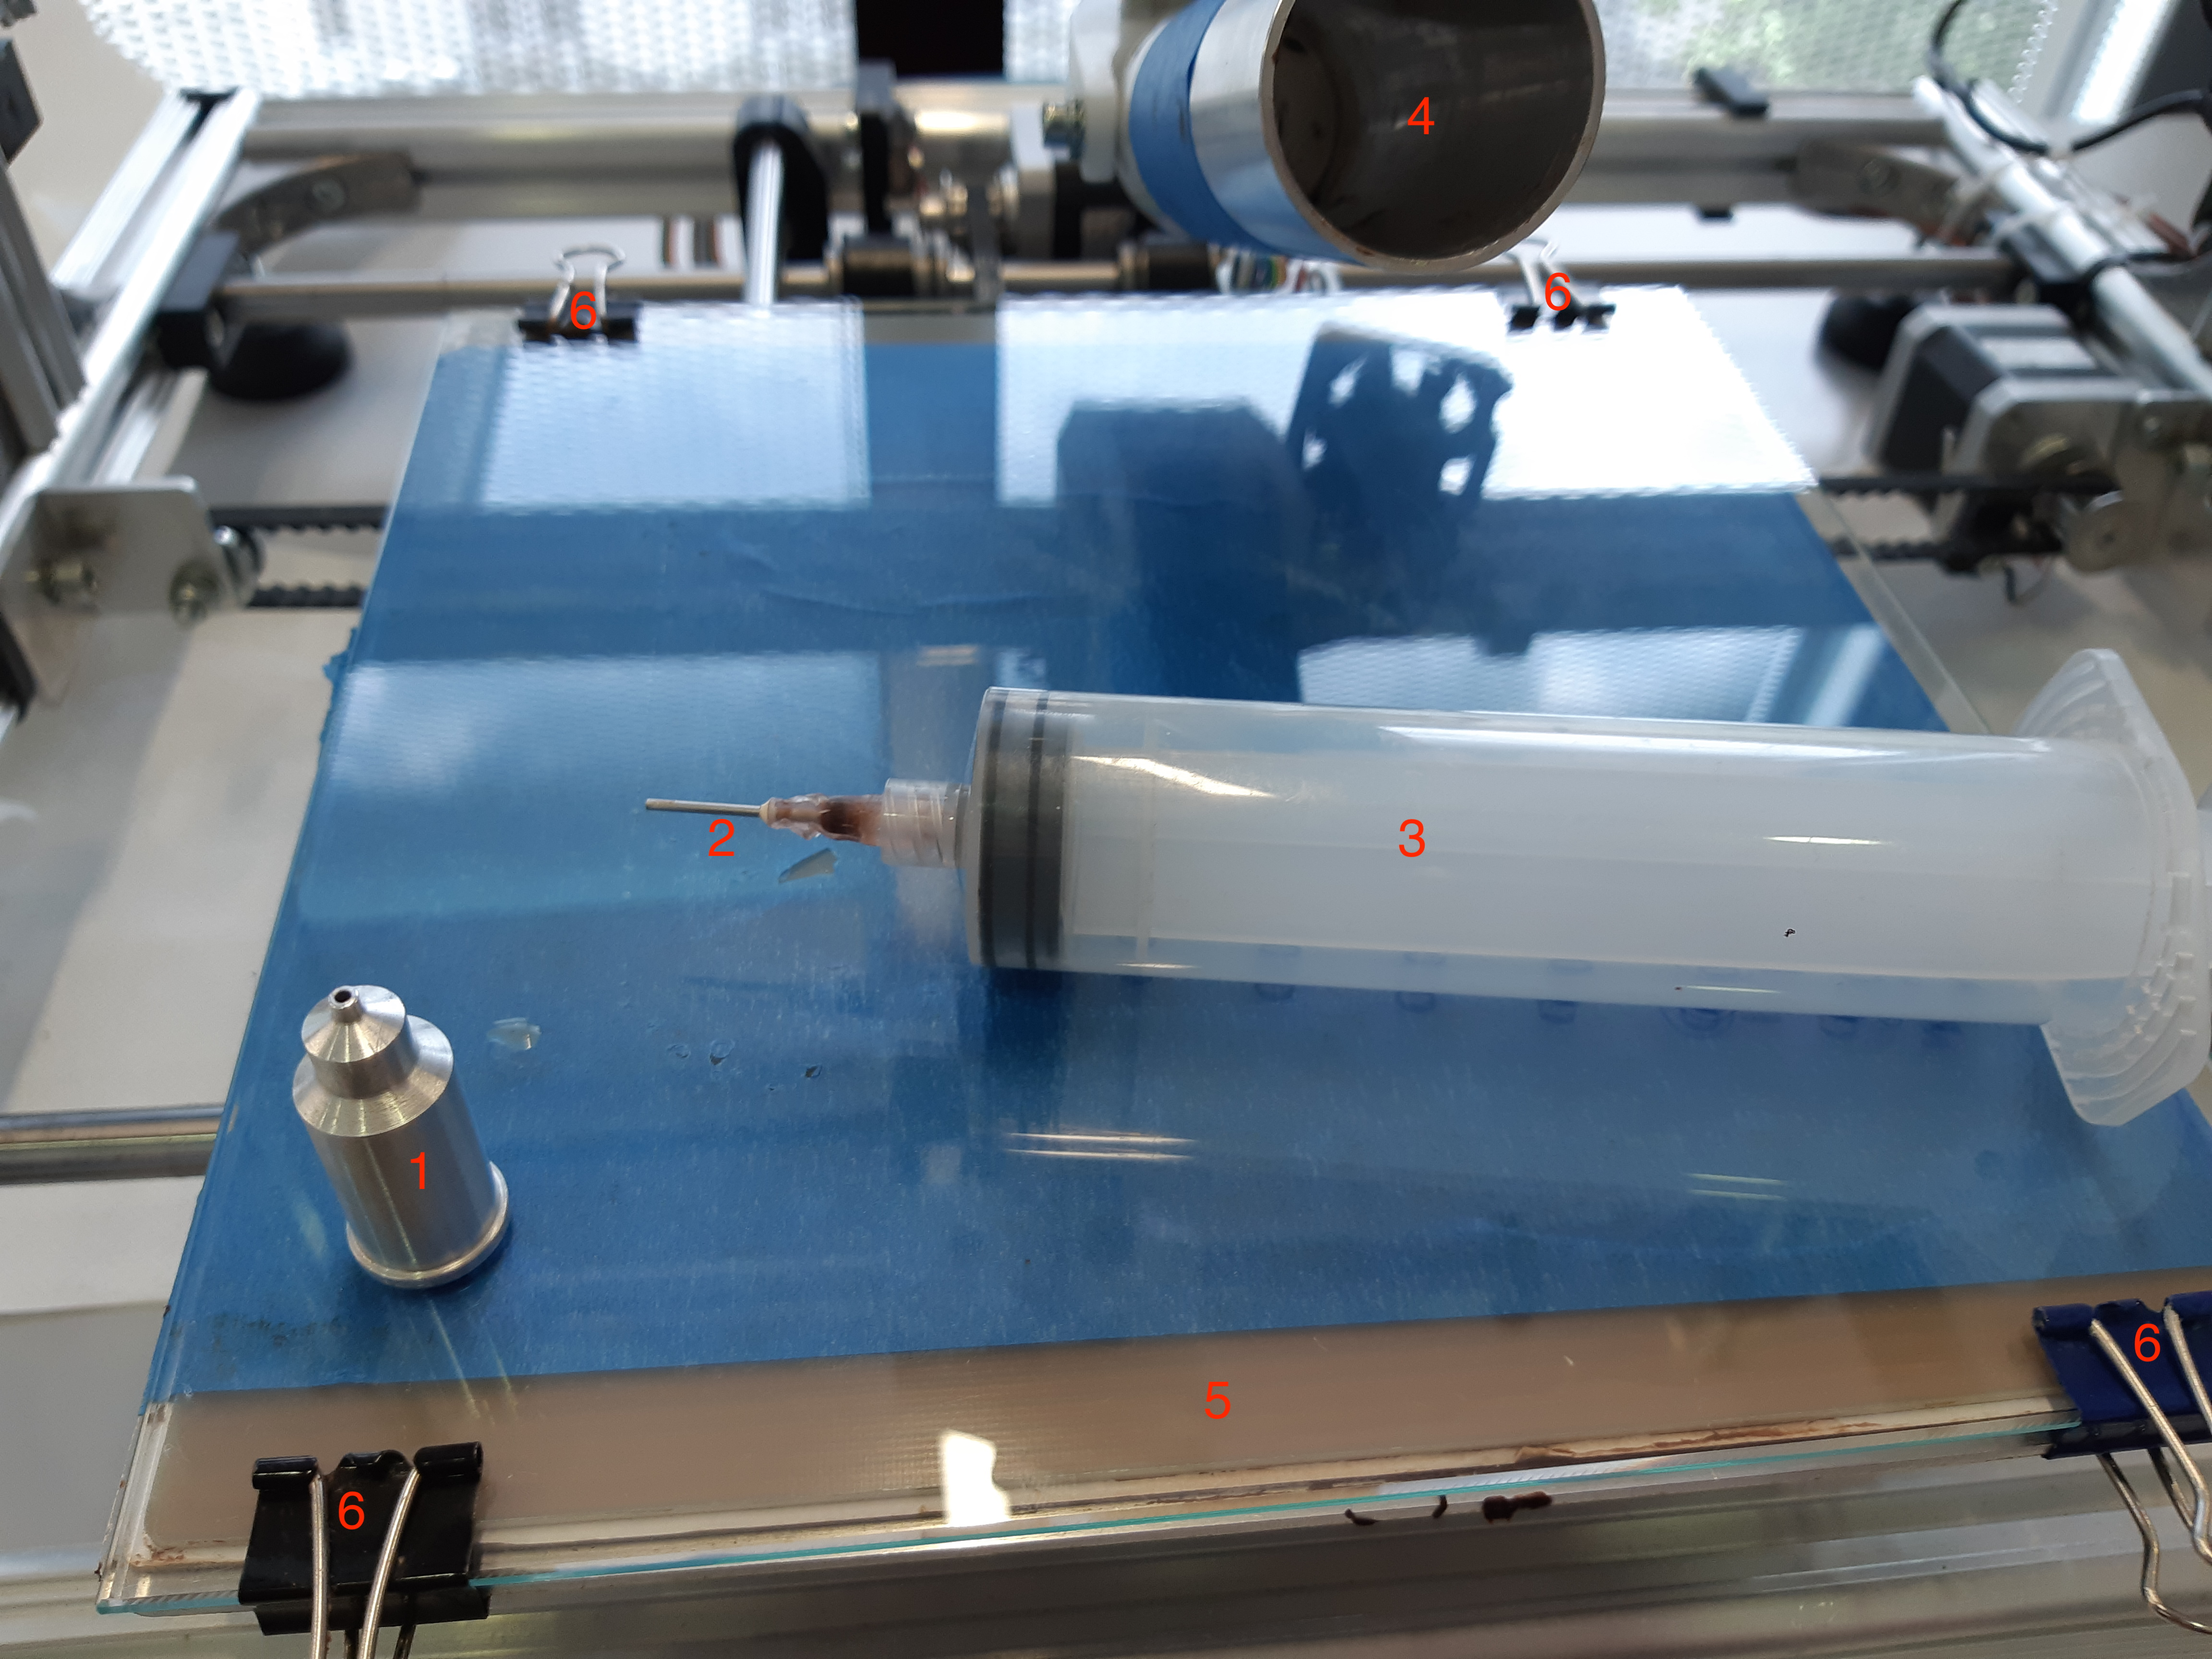
\includegraphics[width=0.9\textwidth]{img/cylinderPieces.jpg}
                \caption*{I componenti del sistema di stampa: tondino (1), ago (2), siringa (3), cilindro portasiringa (4), piatto di vetro (5), clip (6)}
        \end{subfigure}
        \begin{subfigure}{0.5\textwidth}
                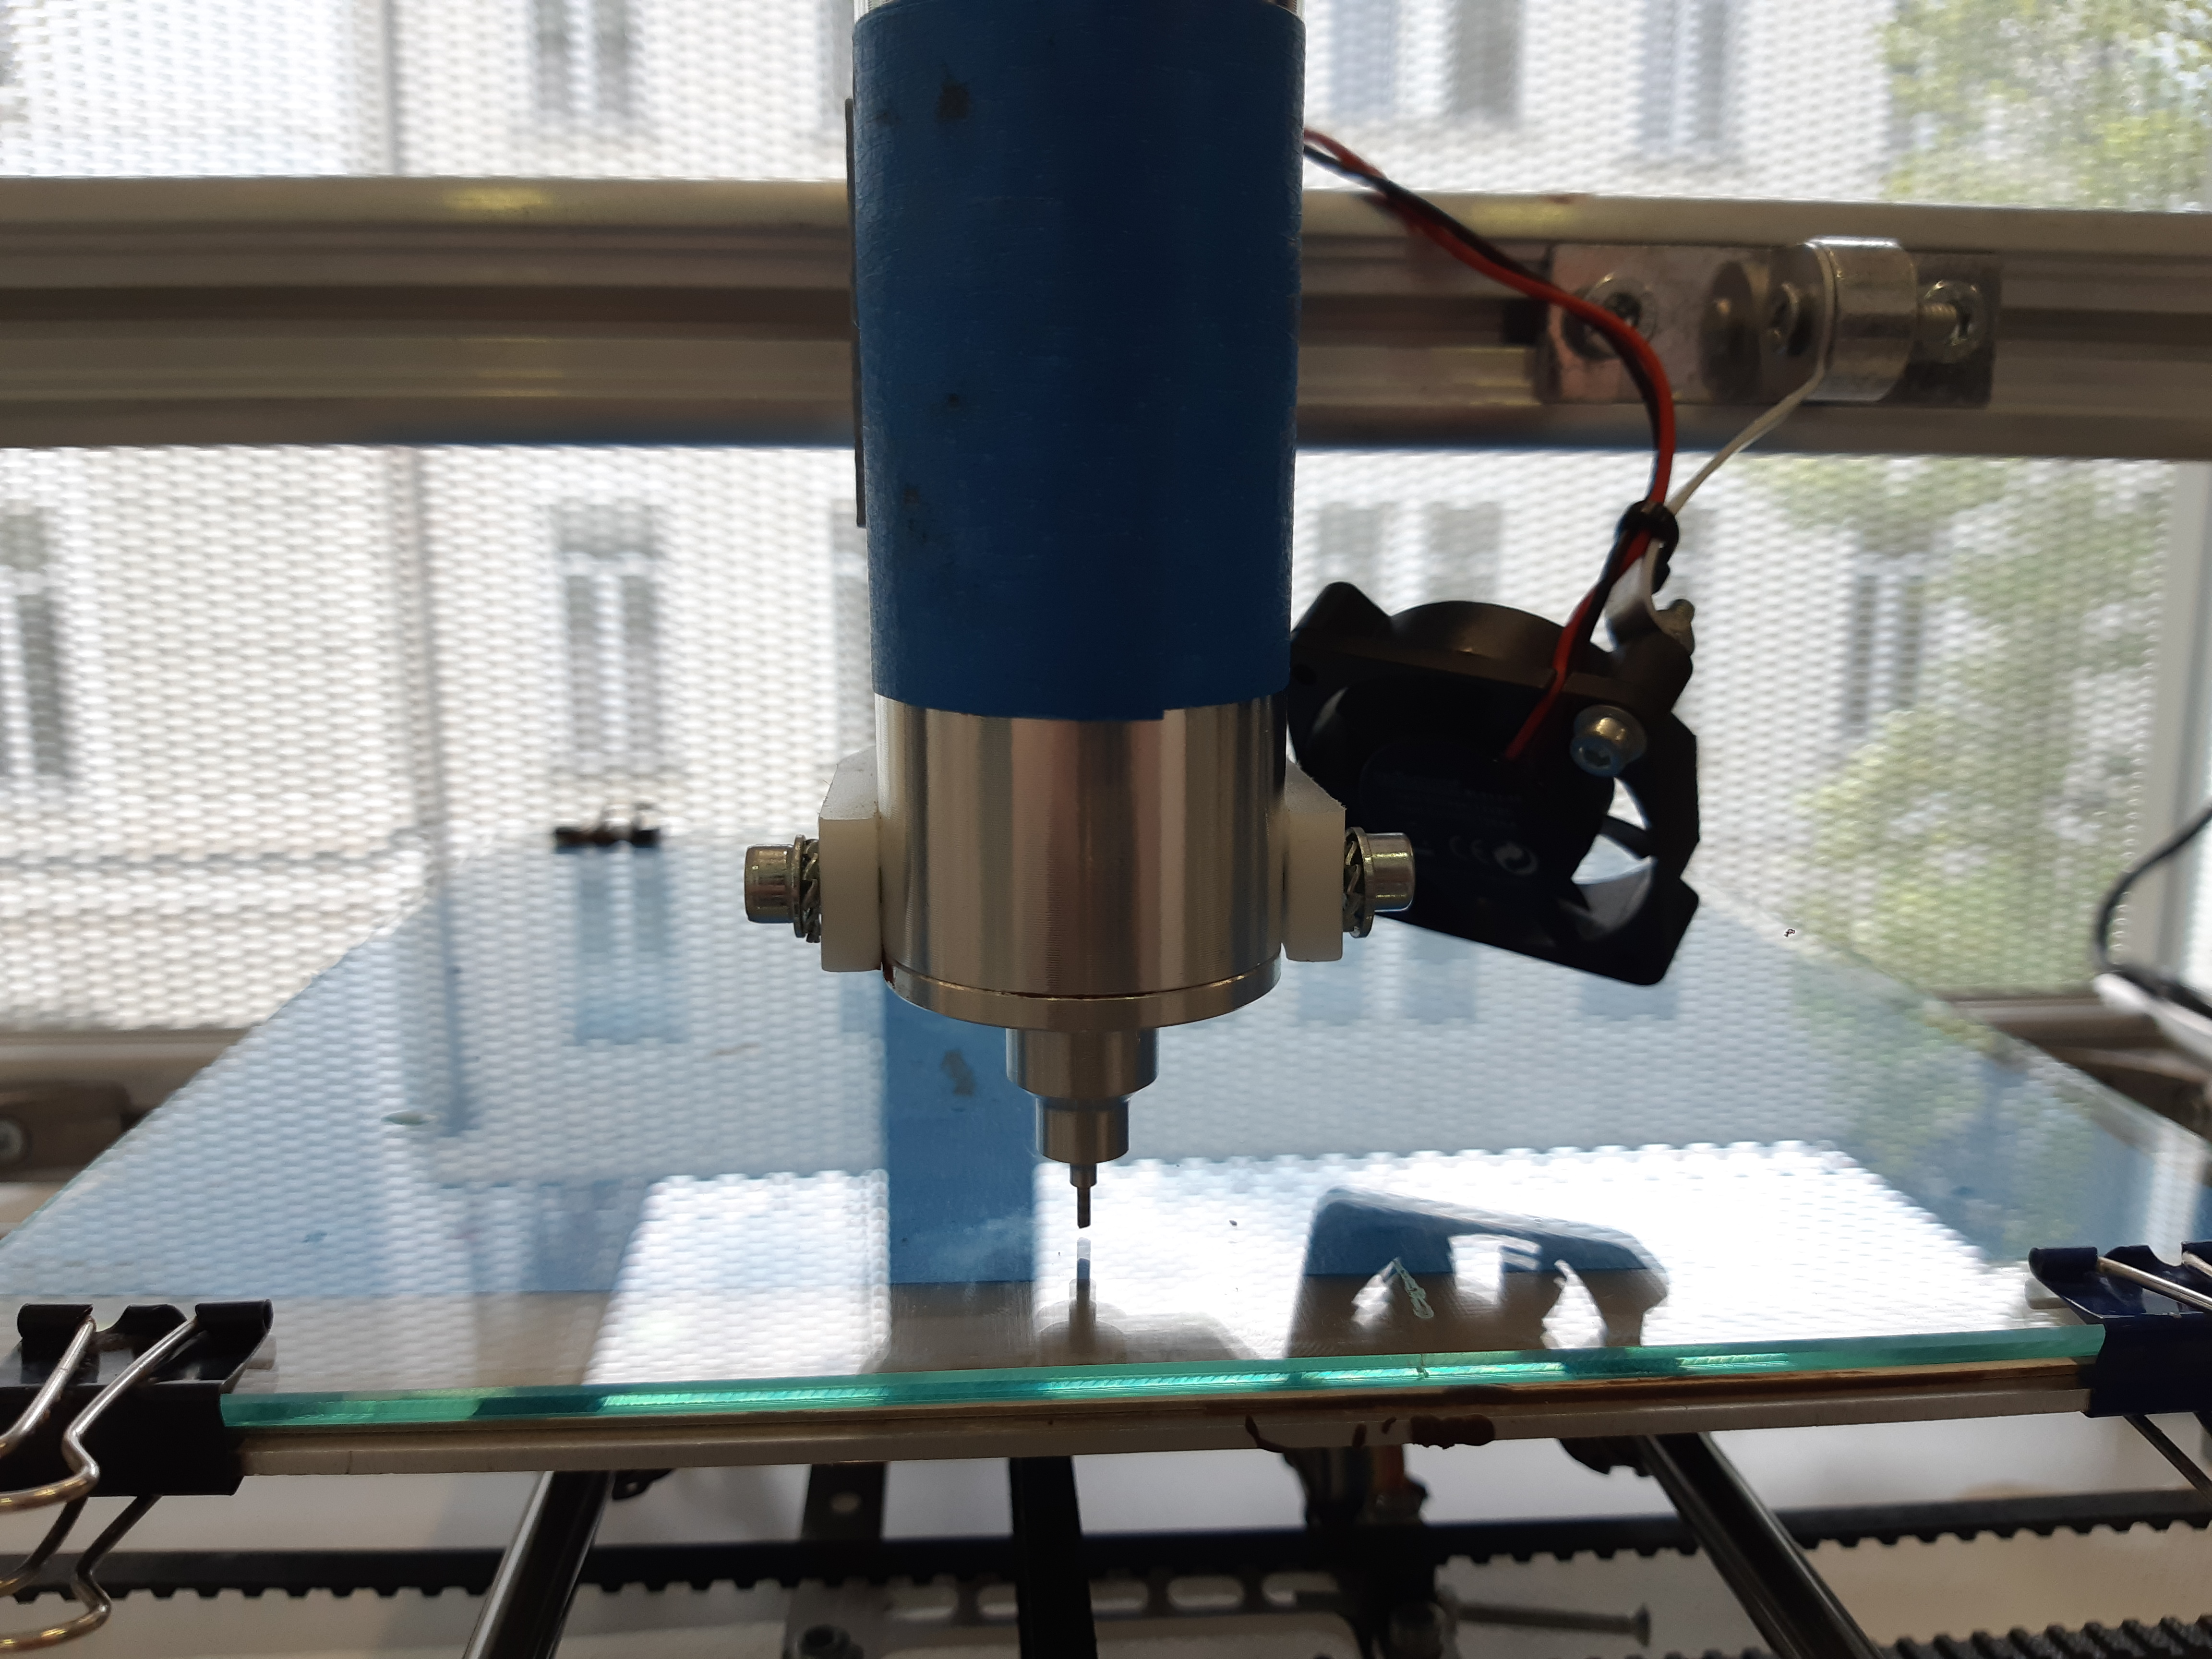
\includegraphics[width=0.9\textwidth]{img/cylinderComplete.jpg}
                \caption*{La siringa assemblata}
         \end{subfigure}
	\end{figure}
	
	\begin{figure}[H]
        \begin{subfigure}{0.5\textwidth}
                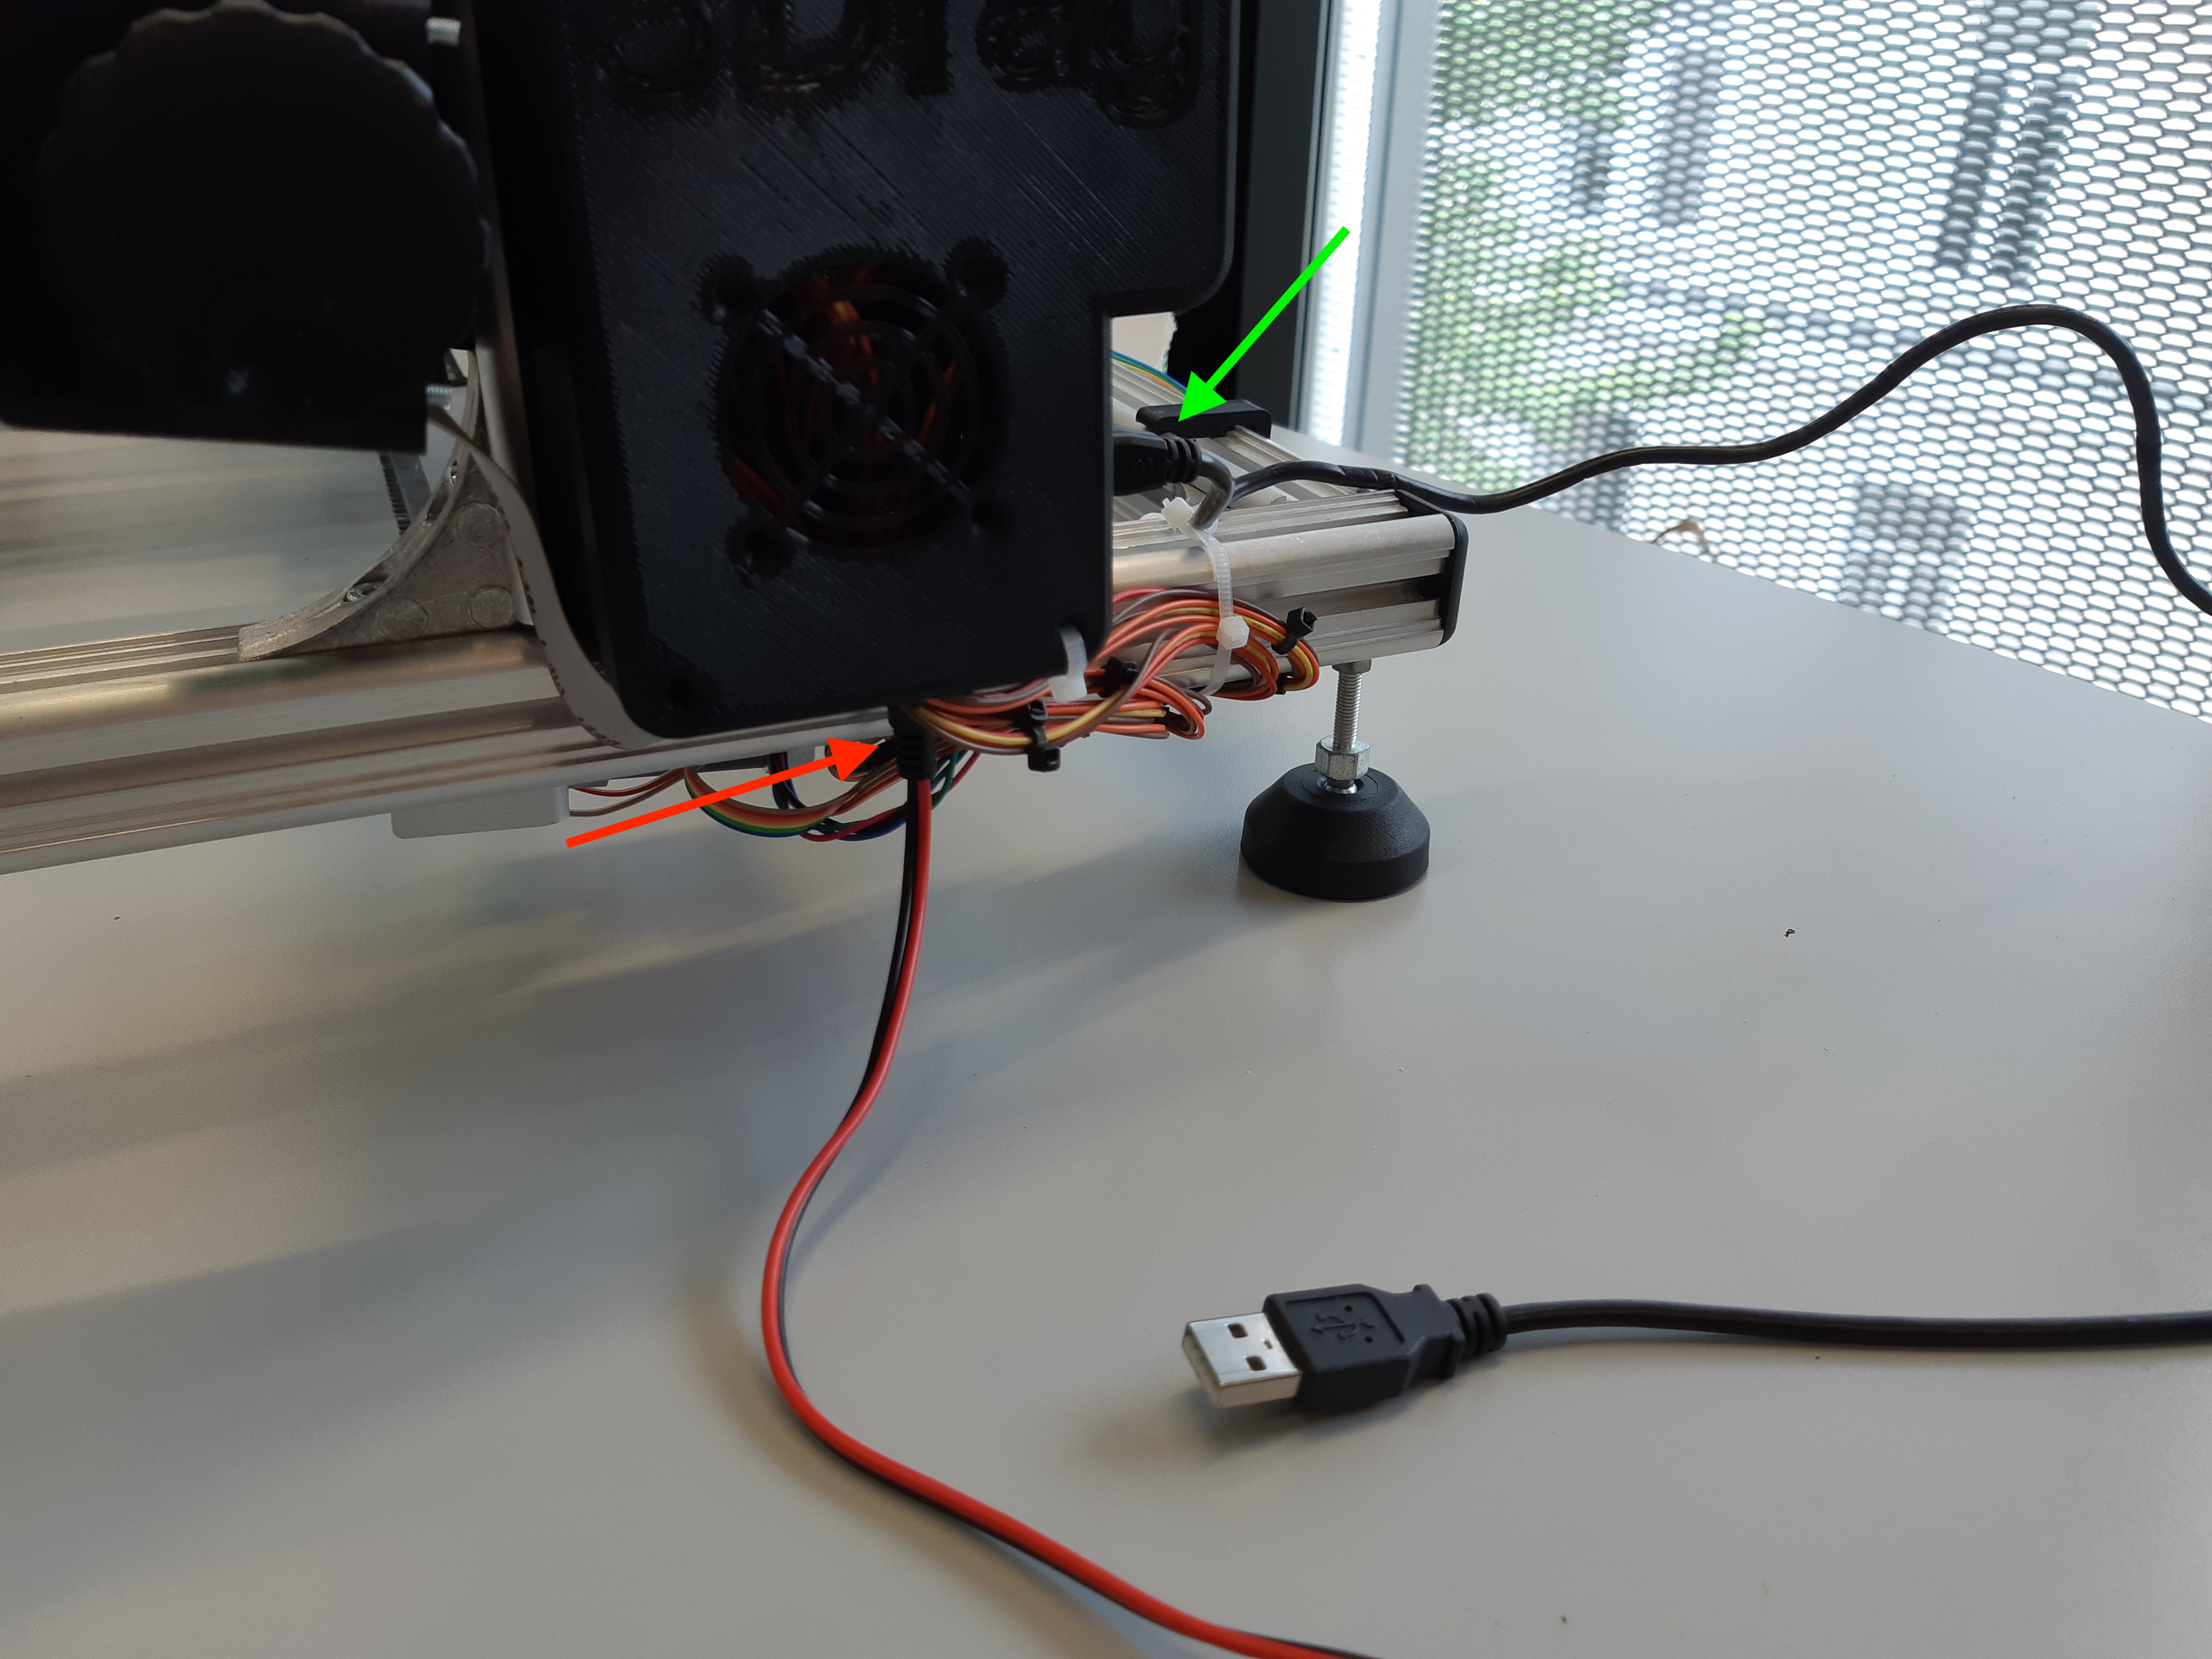
\includegraphics[width=0.9\textwidth]{img/power.jpg}
                \caption*{I cavi della stampante: alimentazione in rosso\\ e USB in verde}
        \end{subfigure}
        \begin{subfigure}{0.5\textwidth}
                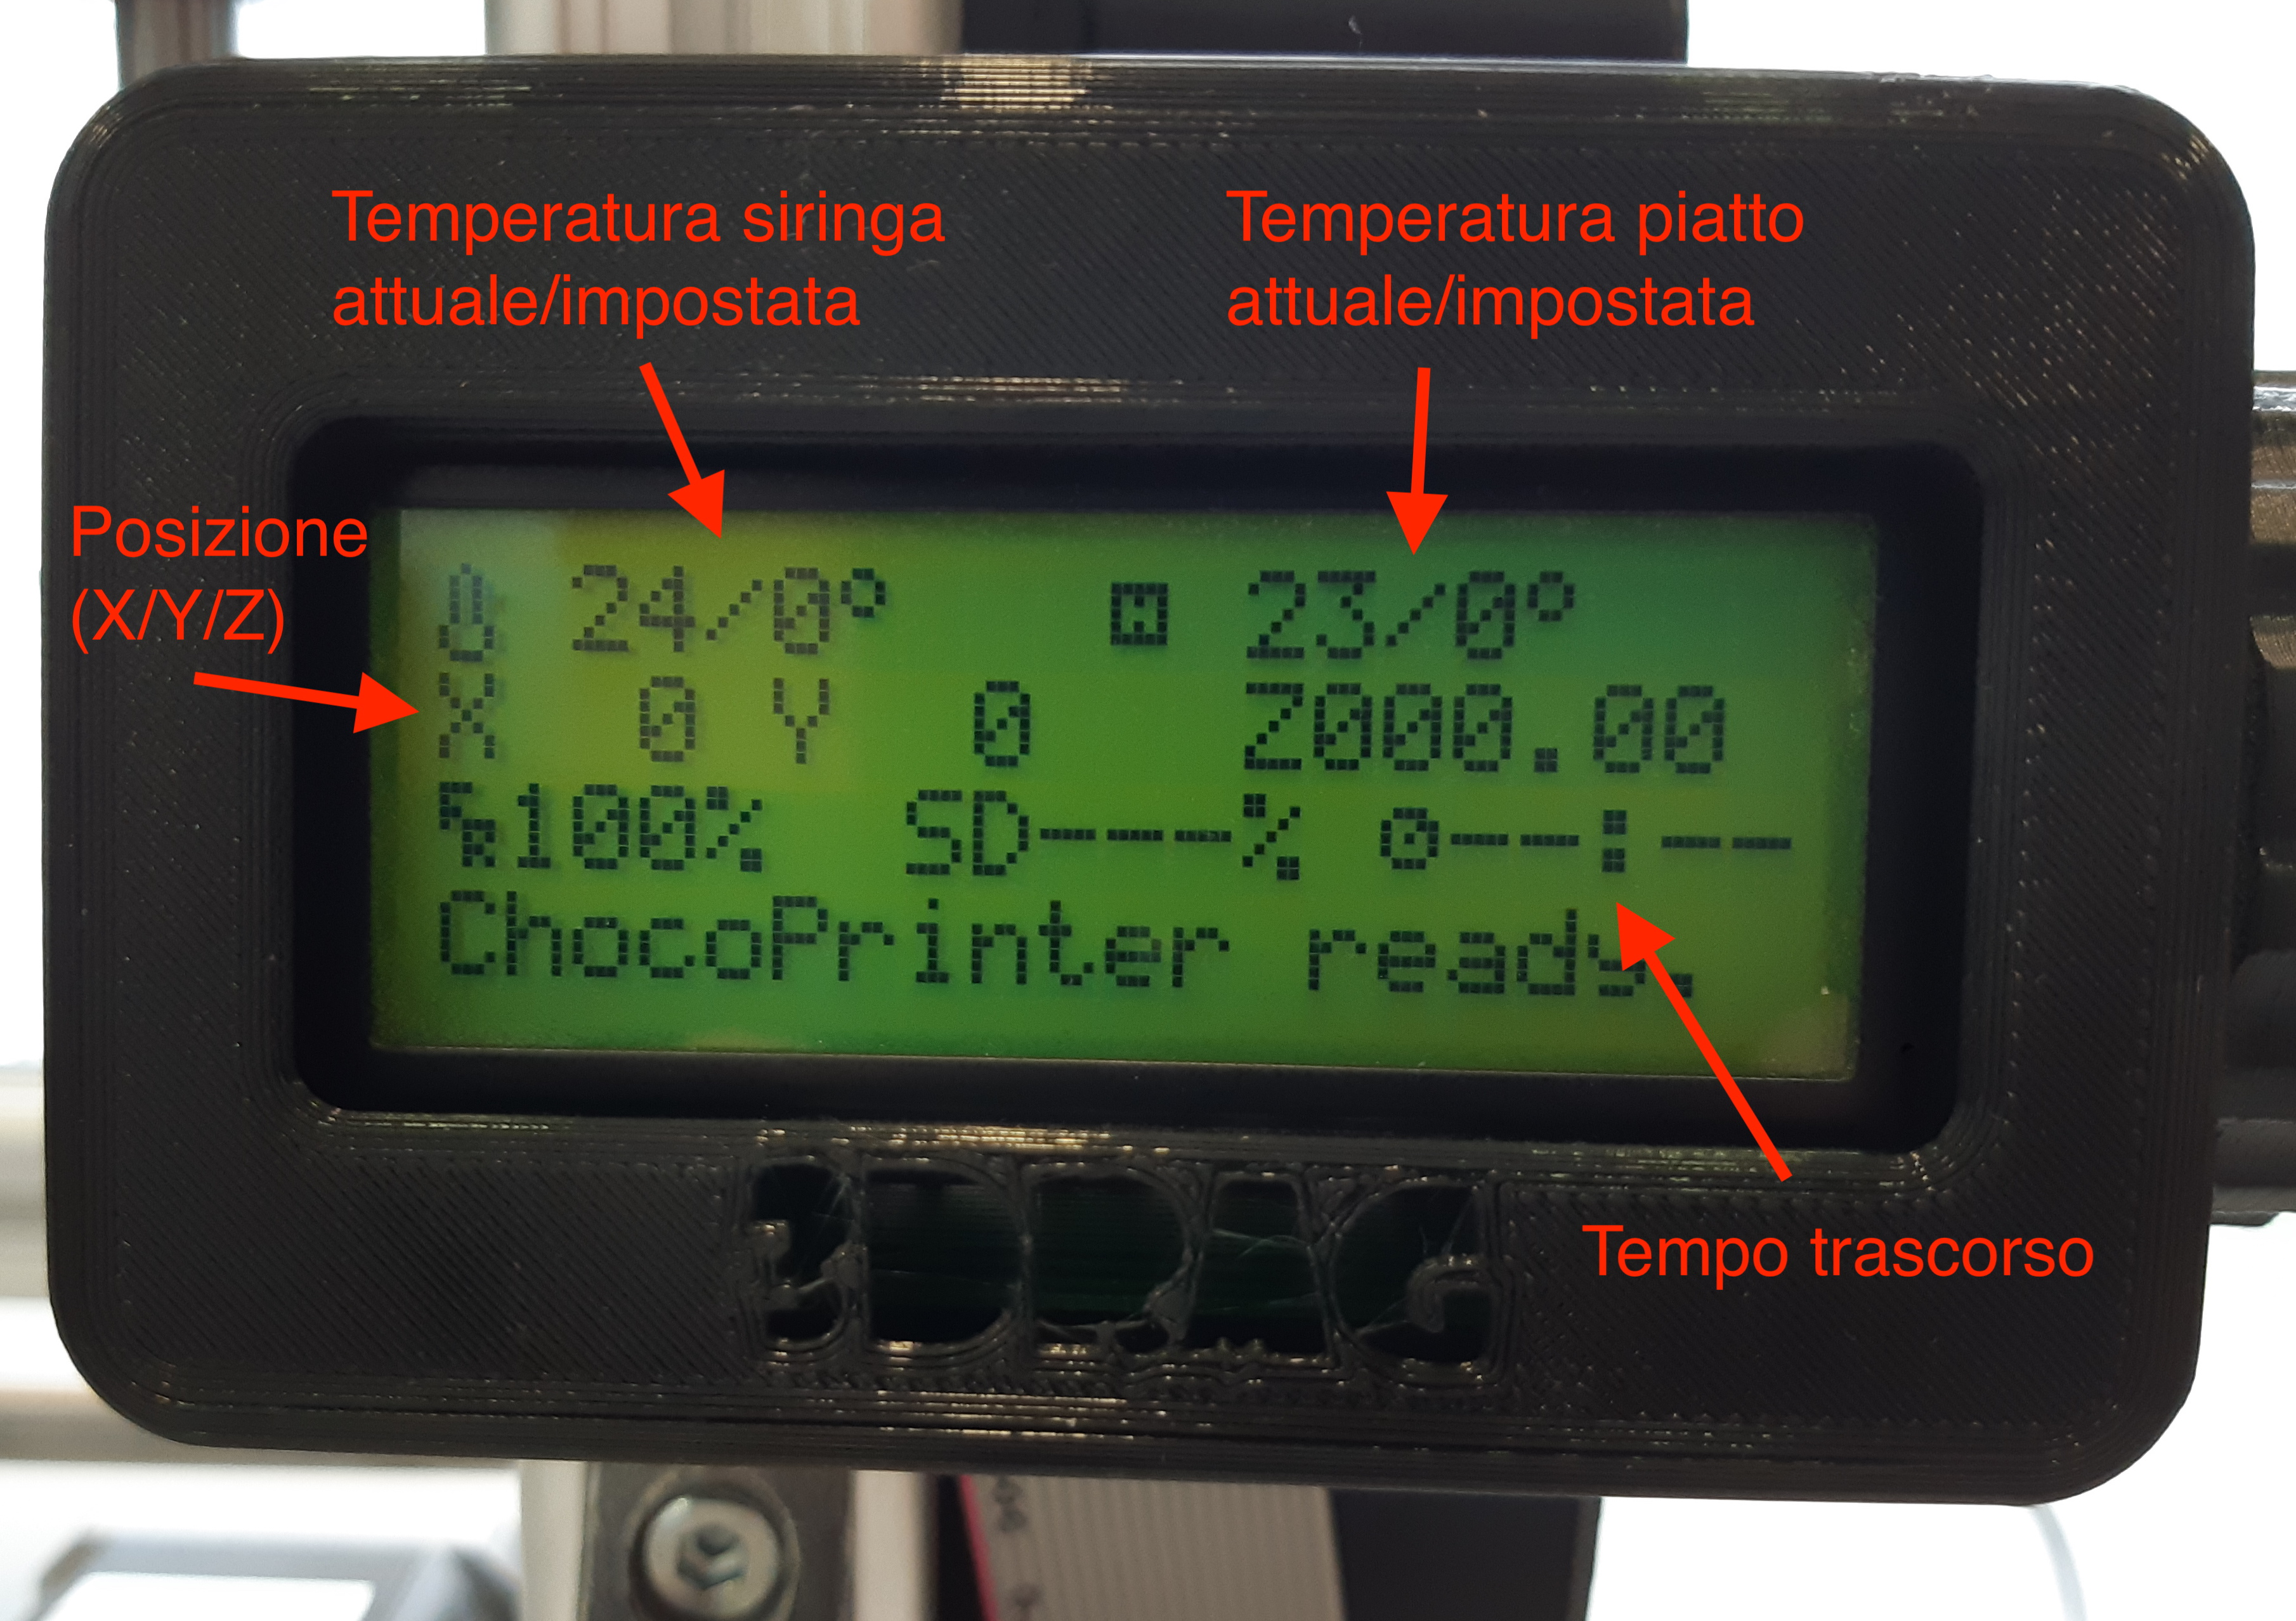
\includegraphics[width=0.9\textwidth]{img/display.jpg}
                \caption*{Il display a riposo}
         \end{subfigure}
	\end{figure}
	
	\begin{figure}[H]
        \begin{subfigure}{0.5\textwidth}
                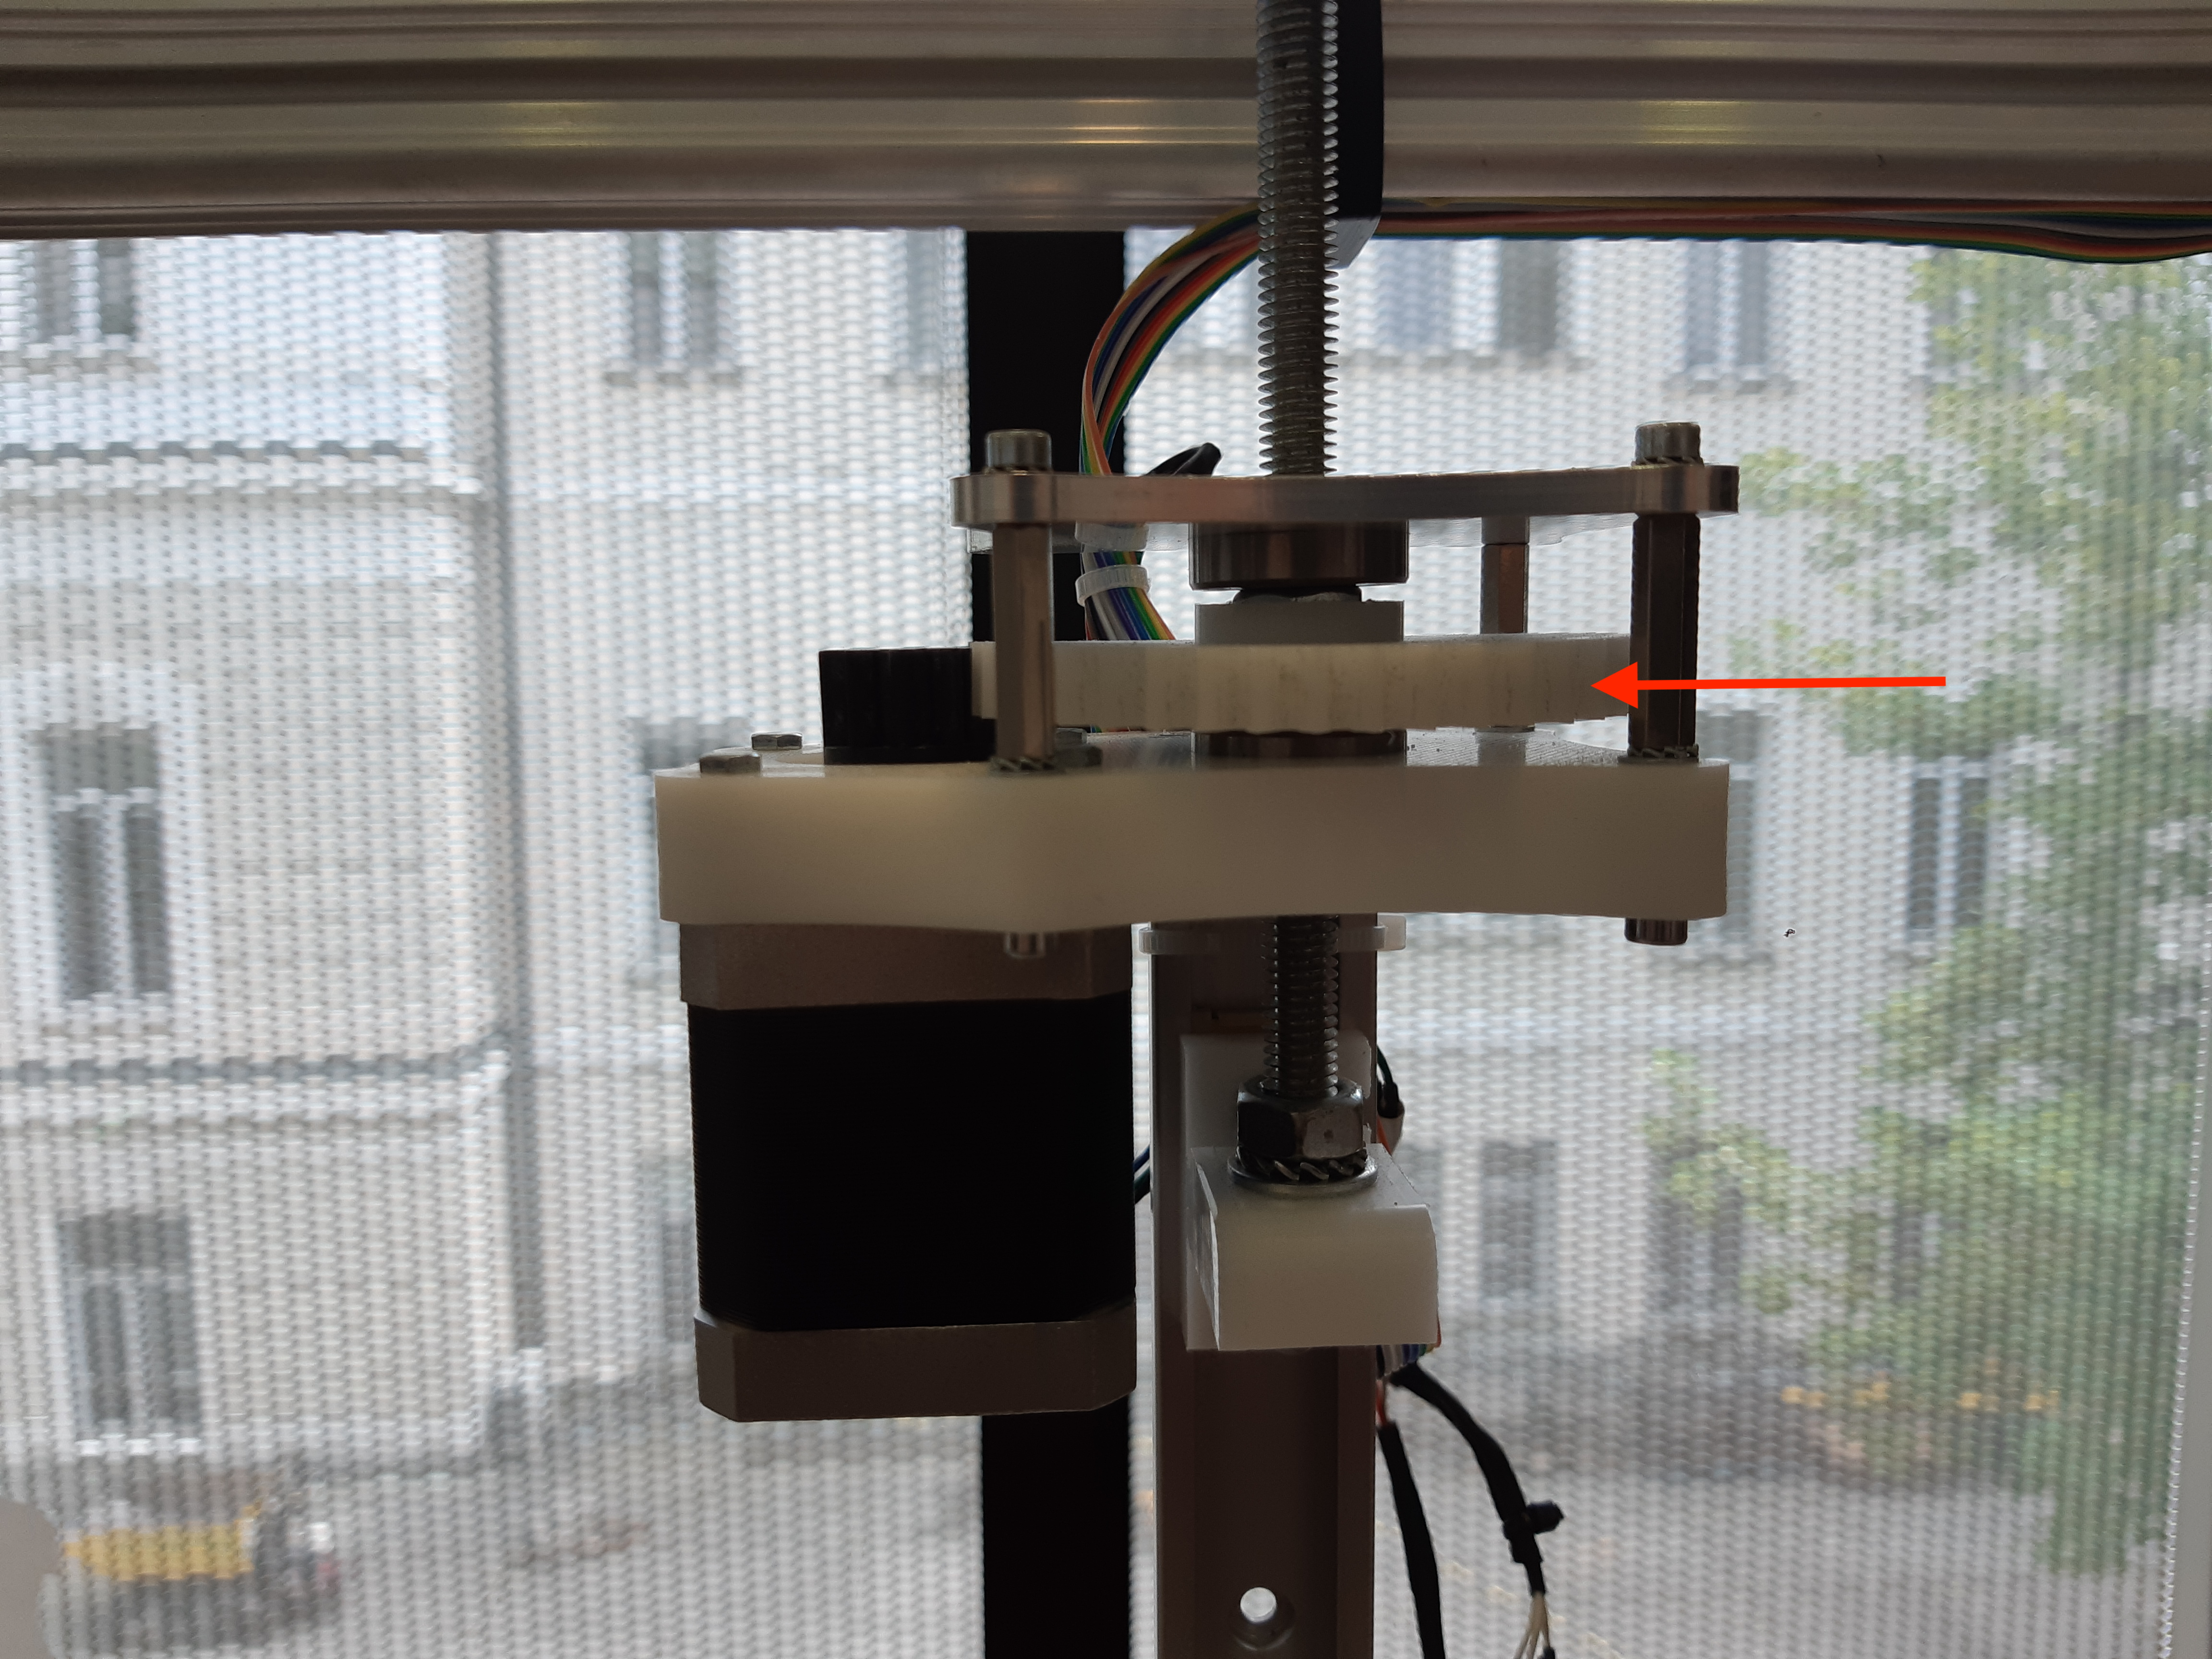
\includegraphics[width=0.9\textwidth]{img/extruder.jpg}
                \caption*{La ruota dentata (freccia) che spinge la siringa}
        \end{subfigure}
        \begin{subfigure}{0.5\textwidth}
                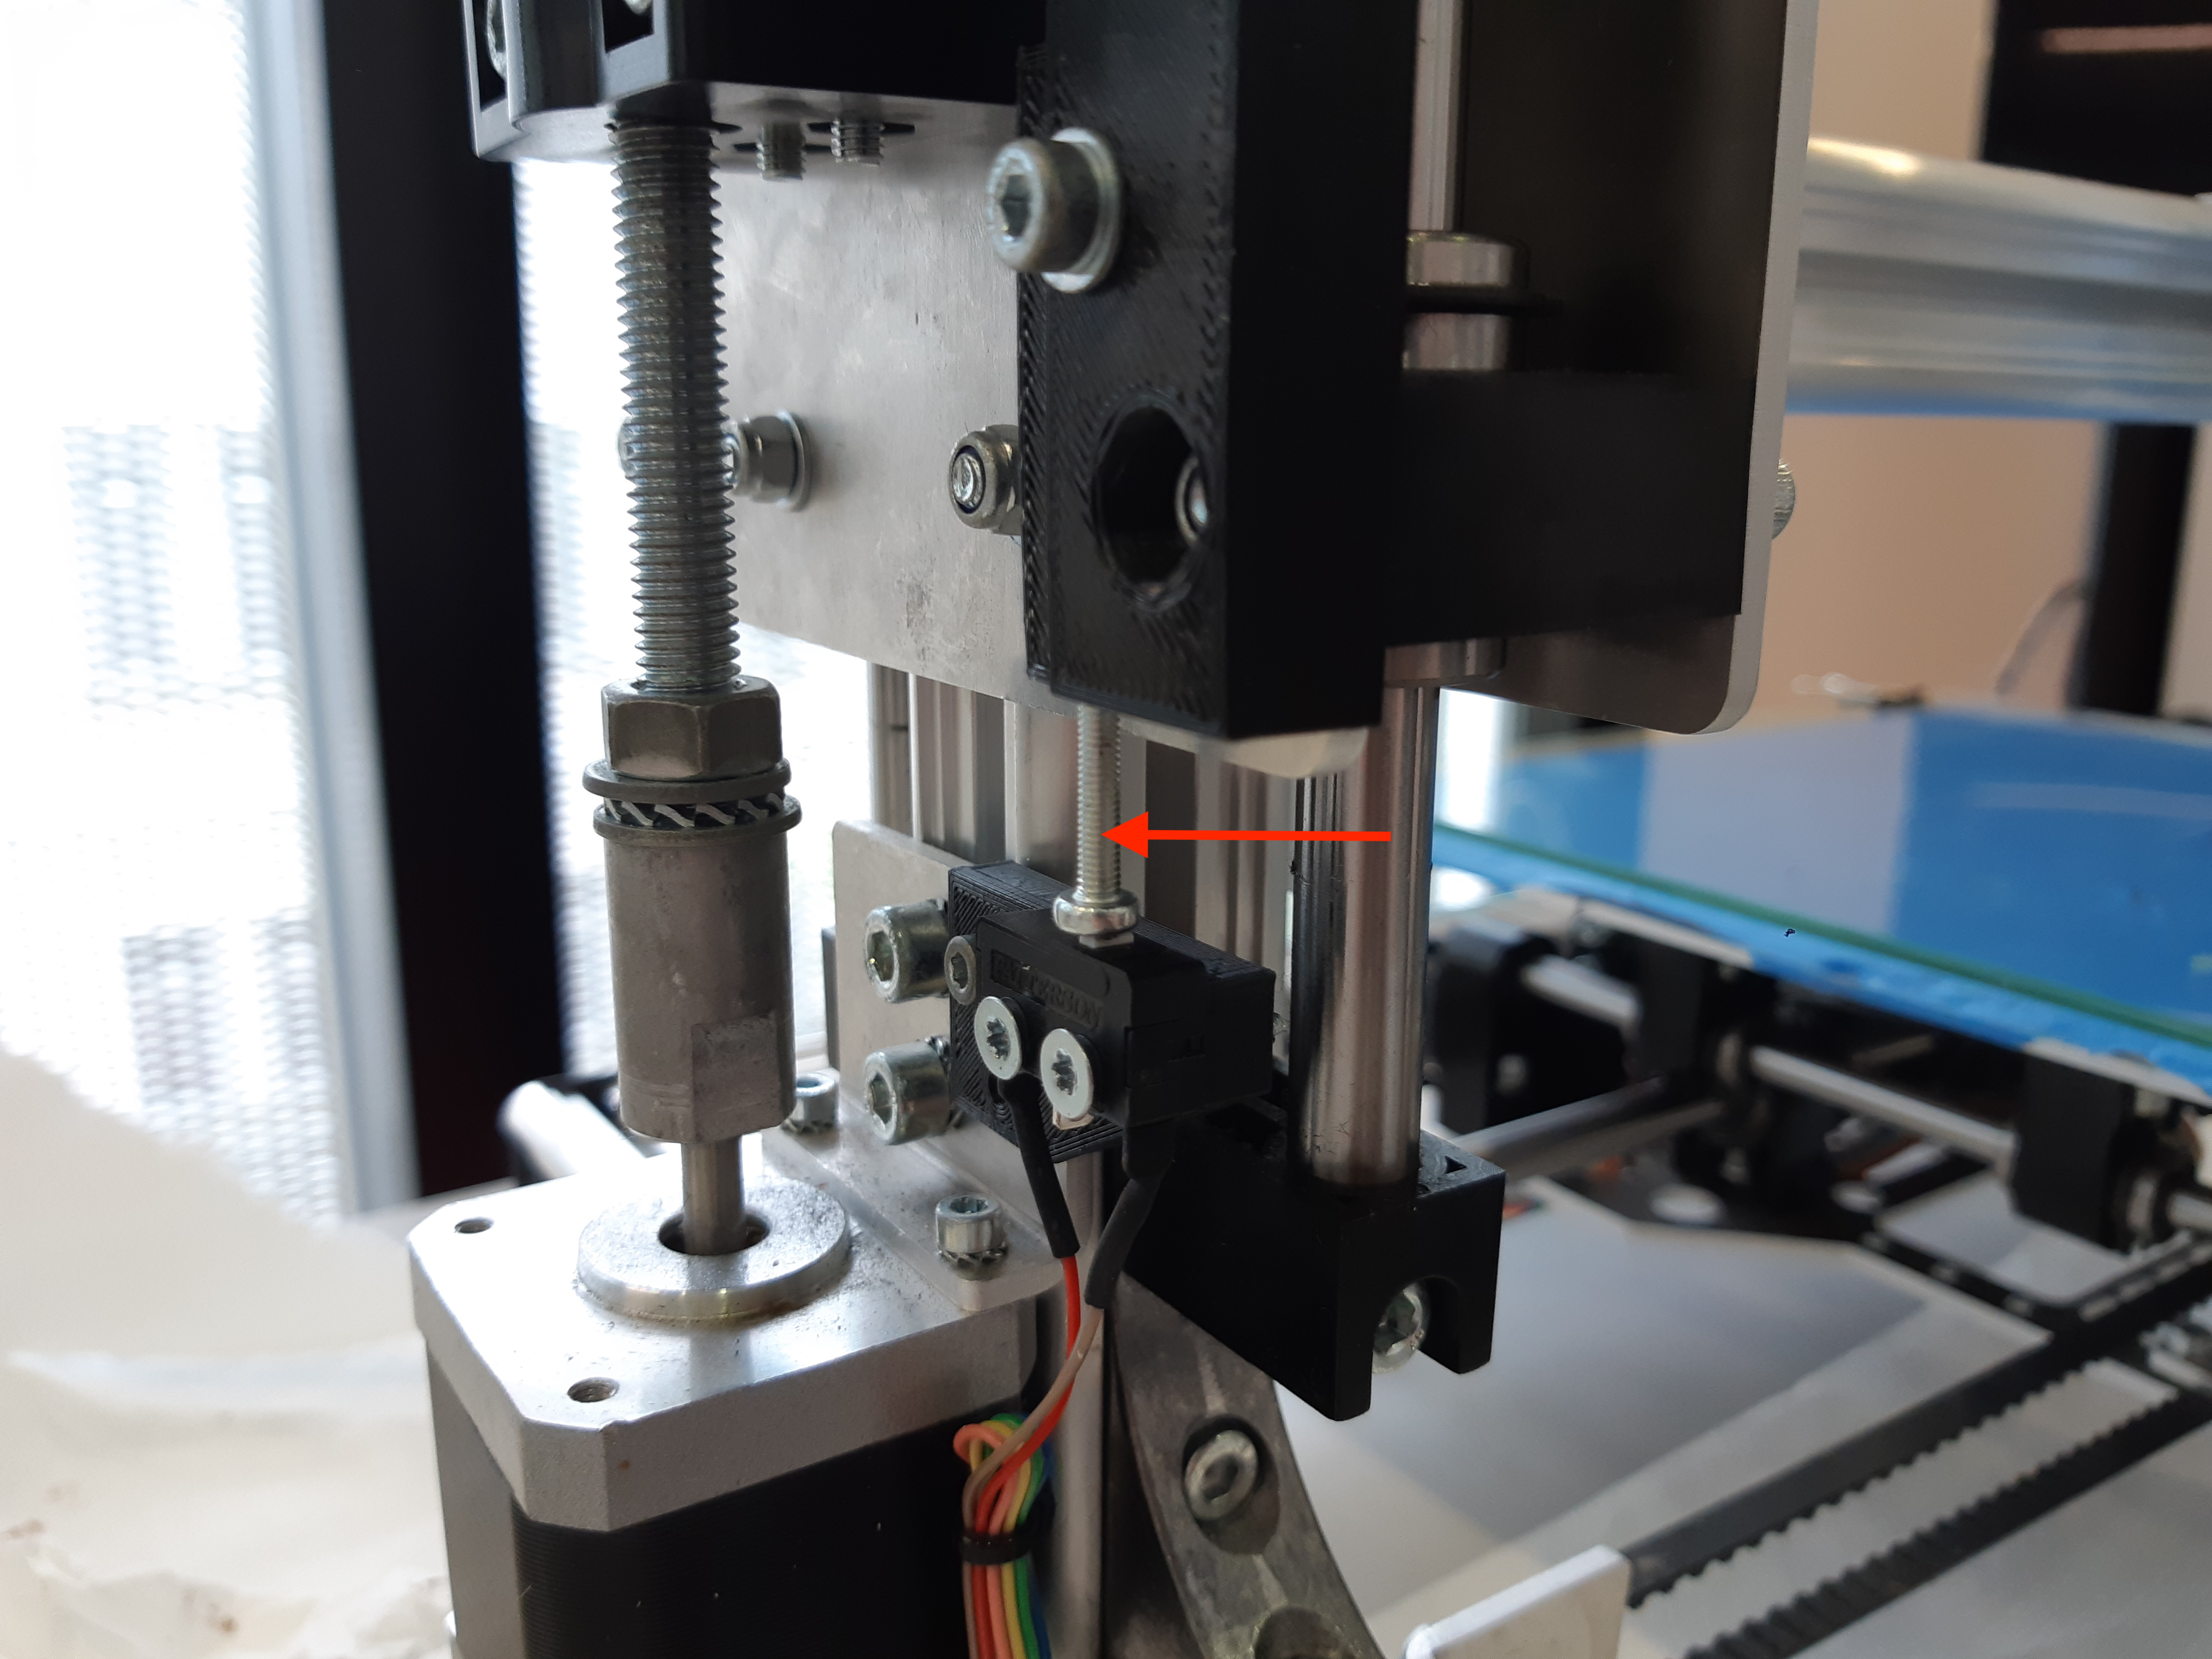
\includegraphics[width=0.9\textwidth]{img/zstop.jpg}
                \caption*{Il sensore z-stop e la vite per regolarlo (freccia)}
         \end{subfigure}
	\end{figure}
	
	\newpage
	

\section{Aggiornamento del firmware}

	Nota: questa procedura richiede una versione 1.0.x di Arduino IDE, che non è compatibile con MacOS da High Sierra 10.13.4 in avanti.

	Scaricare il firmware appropriato (versione 3Drag Choco - LCD alfanumerico, controller verde o nero) dal sito indicato nella sezione \ref{sec:download}.\\
	
	\textbf{IMPORTANTE}: scegliere la versione corretta! Caricare un firmware sbagliato potrebbe rendere la stampante inutilizzabile!\\
	
	Estrarre il pacchetto del firmware ed aprire il file \texttt{Marlin.ino} nella cartella \texttt{Marlin}. Dal menu \texttt{Sketch > Import Library...} scegliere \texttt{Add Library...} e selezionare la cartella \texttt{libraries/U8glib} nella cartella scaricata in precedenza.
	Dal menu \texttt{Tools > Board} selezionare \texttt{Arduino Mega 2560 or Mega ADK} e dal menu \texttt{Tools > Serial Port} selezionare la porta COM associata alla stampante. Verificare sulla scheda della stampante che il jumper JPROG sia inserito. Cliccare sul secondo pulsante da sinistra (\texttt{Upload}) e attendere il completamento della procedura. 
	A procedura terminata, scollegare cavo USB e alimentazione della stampante e rimuovere il jumper.

\end{document}